\documentclass{beamer}
\usetheme{metropolis}
\usepackage{enumitem}

\graphicspath{{media/}}
\usepackage{booktabs} % Required for better table rules
\usepackage{multicol}
%Information to be included in the title page:
\setbeamertemplate{frame footer}{\insertdate{} - \insertshortauthor{}}
\title{Mininet}
\author{Manuel Dias}
\institute{UCLouvain}
\date{16/05/2025}

\begin{document}

\frame{\titlepage}


\begin{frame}
\frametitle{Network Scan}
\begin{columns}
    % Column 1
    \begin{column}{0.5\textwidth}
        \Large Attack
        \begin{figure}
            \centering
            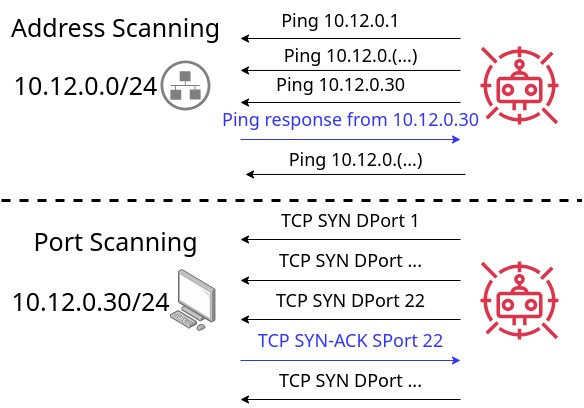
\includegraphics[width=0.8\textwidth]{scan_attack.jpg}\\
        \end{figure}
            \begin{itemize}[label={}]
                \item \footnotesize Send ICMP Requests to all the addresses of a given sub-domain
                \item \footnotesize Send TCP SYN packets to all of the found Hosts that responded
               \item \footnotesize  Save the addresses and their open ports
            \end{itemize}
    \end{column}
    % Column 2
    \begin{column}{0.5\textwidth}
        \Large Defense
        \begin{figure}
            \centering
            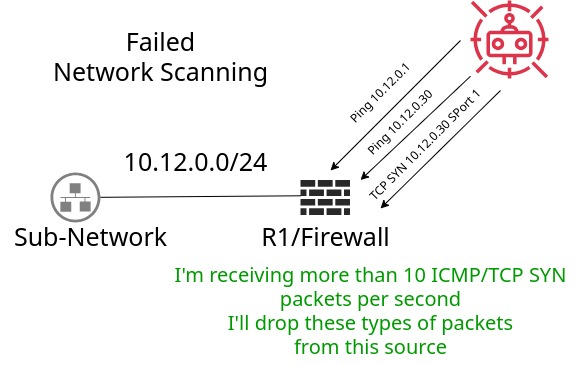
\includegraphics[width=0.8\textwidth]{scan_defense.jpg}\\
        \end{figure}
            \begin{itemize}[label={}]
                \item \footnotesize Send ICMP Requests/TCP SYN Packets to all the addresses of a given sub-domain
                \item \footnotesize Firewall sees that the amount of these type of packets that were received surpasses the threshold so it drops
            \end{itemize}
    \end{column}
\end{columns}
\end{frame}

\begin{frame}
\frametitle{Dns Reflection}
\begin{columns}
    % Column 1
    \begin{column}{0.5\textwidth}
        \Large Attack
        \begin{figure}
            \centering
            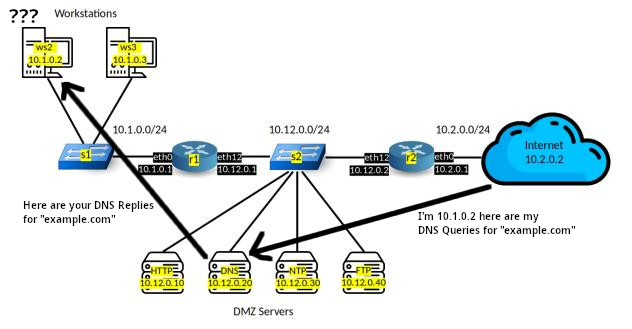
\includegraphics[width=\textwidth]{dns_attack.jpg}\\
        \end{figure}
            \begin{itemize}[label={}]
                \item \footnotesize Send Dns Requests in the name of the victim
                \item \footnotesize DNS Server processes and sends response to the victim
                \item \footnotesize Victim is overloaded with Traffic becoming Unavailable
            \end{itemize}
    \end{column}
    % Column 2
    \begin{column}{0.5\textwidth}
        \Large Defense
        \begin{figure}
            \centering
            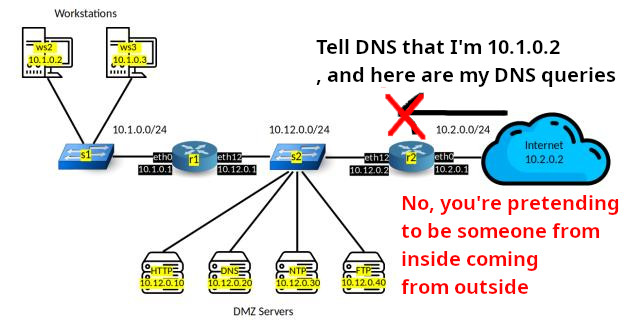
\includegraphics[width=\textwidth]{dns_defense.jpg}\\
        \end{figure}
            \begin{itemize}[label={}]
                \item \footnotesize Send Dns Requests in the name of the victim
                \item \footnotesize R2 Blocks outside traffic coming from spoofed internal IP's
                \item \footnotesize R1 sets a limit rate for DNS Responses
            \end{itemize}
    \end{column}
\end{columns}
\end{frame}

\begin{frame}
\frametitle{Arp Poisoning}
\begin{columns}
    % Column 1
    \begin{column}{0.5\textwidth}
        \\
        \Large Attack
        \begin{figure}
            \centering
            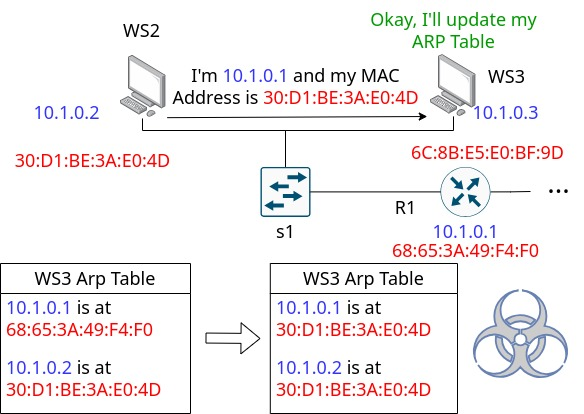
\includegraphics[width=0.8\textwidth]{arp_attack.jpg}\\
        \end{figure}
            \begin{itemize}[label={}]
                \item \footnotesize Send Spoofed ARP packet saying that our MAC Address matches the Default Gateway's
                \item \footnotesize Victim Updates it's ARP Table with wrong MAC Address
               \item \footnotesize Attacker receiver all the traffic coming out of Victim
            \end{itemize}
    \end{column}
    % Column 2
    \begin{column}{0.5\textwidth}
        \Large Defense
        \begin{figure}
            \centering
            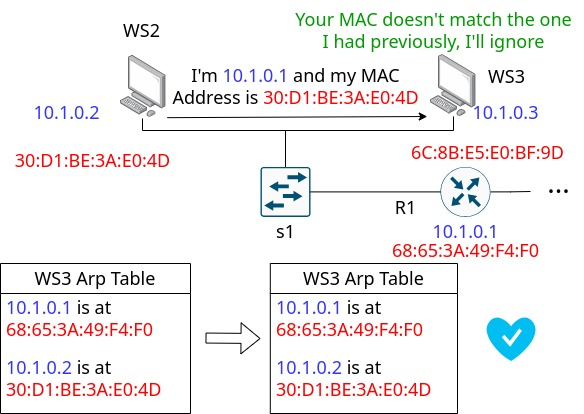
\includegraphics[width=0.8\textwidth]{arp_defense.jpg}\\
        \end{figure}
            \begin{itemize}[label={}]
                \item \footnotesize Send Spoofed ARP packet saying that our MAC Address matches the Default Gateway's
                \item \footnotesize Victim checks it's ARP Table for changes in the MAC
                \item \footnotesize Ignores the ARP Change request
            \end{itemize}
    \end{column}
\end{columns}
\end{frame}


\begin{frame}
\frametitle{Syn Flooding}
\begin{columns}
    % Column 1
    \begin{column}{0.5\textwidth}
        \Large Attack
        \begin{figure}
            \centering
            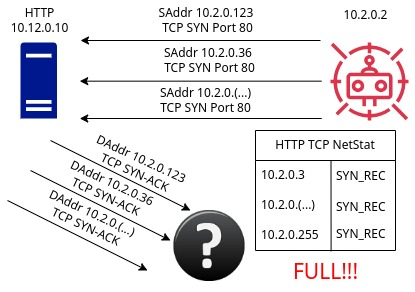
\includegraphics[width=0.8\textwidth]{flood_attack.jpg}\\
        \end{figure}
            \begin{itemize}[label={}]
                \item \footnotesize Send spoofed TCP SYN packets to a victim's open port
                \item \footnotesize Victim adds the tcp connections
                \item \footnotesize Victim sends SYN-ACKS that will never get be answered leaving the connections table full
            \end{itemize}
    \end{column}
    % Column 2
    \begin{column}{0.5\textwidth}
        \\
        \Large Defense
        \begin{figure}
            \centering
            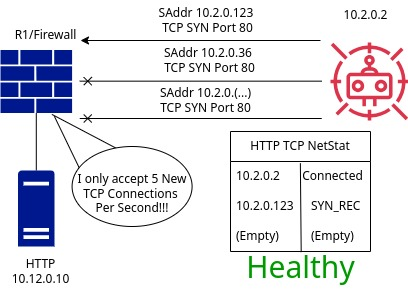
\includegraphics[width=0.8\textwidth]{flood_defense.jpg}\\
        \end{figure}
            \begin{itemize}[label={}]
                \item \footnotesize Send spoofed TCP SYN packets to a victim's open port
                \item \footnotesize Firewall sets a limit of 5 new TCP Connections per second
                \item \footnotesize Victim might send unanswerable SYN-ACKS but not enough to block new legitimate connections
            \end{itemize}
    \end{column}
\end{columns}
\end{frame}

\begin{frame}
\frametitle{SSH Bruteforce}
\begin{columns}
    % Column 1
    \begin{column}{0.5\textwidth}
        \Large Attack
        \begin{figure}
            \centering
            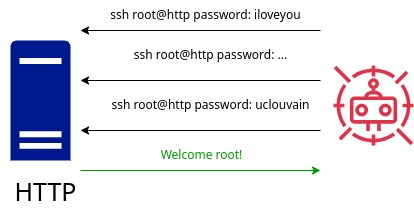
\includegraphics[width=0.8\textwidth]{brute_attack.jpg}\\
        \end{figure}
            \begin{itemize}[label={}]
                \item \footnotesize Try to ssh login with every password in a list
                \item \footnotesize Eventually find correct credentials
                \item \footnotesize Login and profit
            \end{itemize}
    \end{column}
    % Column 2
    \begin{column}{0.5\textwidth}
        \\~\\
        \Large Defense
        \begin{figure}
            \centering
            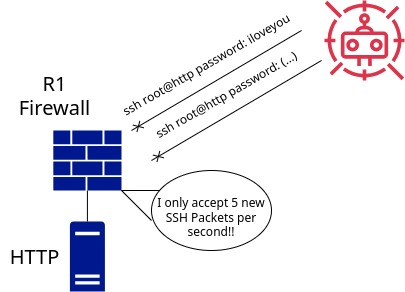
\includegraphics[width=0.8\textwidth]{brute_defense.jpg}\\
        \end{figure}
            \begin{itemize}[label={}]
                \item \footnotesize Try to ssh login with every password in a list
                \item \footnotesize Firewall blocks the attempt because it surpasses the threshold
            \end{itemize}
    \end{column}
\end{columns}
\end{frame}
\end{document}
